\chapter{Evaluácia výsledkov}

\paragraph{}
V predošlej kapitole sme bližšie popísali implementáciu našich algoritmov. Táto kapitola sa zameriava na evaluáciu výsledkov týchto algoritmov. Keďže práca sa zaoberá implementáciou algoritmov na generovanie hesiel pomocou vstupného slovníka, bolo potrebné si nájsť vhodný vstupný slovník. Podarilo sa nám nájsť online zdroj slovníkov \cite{dictionaries}, ktorý obsahuje slovníky s usporiadanými heslami podľa pravdepodobnosti výskytu. Slovník je formátovaný v dvoch stĺpcoch, kde prvý obsahuje informáciu o počte výskytov daného heslá a druhý je samotné heslo.

\paragraph{}
Testy boli spúšťané na procesore Intel® Core™ i5-4690K s rýchlosťou 3.50GHz so 16 gigabajtami operačnej pamäte na operačnom systéme Windows 10. Implementácia jednotlivých algoritmov bola písaná v jazyku Python 3.5.1 a spúšťaná 64-bitovou verziou interpretéra.

\section{Časová náročnosť}
\label{sec:time}
V tomto základnom teste sme merali čas behu algoritmov pre jednotlivé parametre spustenia. Pre všetky testy používame slovník \emph{\href{http://downloads.skullsecurity.org/passwords/rockyou-withcount.txt.bz2}{rockyou-withcount}} stiahnutý z nášho zdroja slovníkov \cite{dictionaries}. Slovník sme upravovali aby obsahoval len heslá zodpovedajúce maximálnej dĺžke hesiel, ktoré generuje bezkontextová gramatika. Týmto sme znížili pravdepodobnosť Markovovského zdroja generovať heslá dlhšie ako stanovené maximum pre gramatiku ako je vidieť na grafe \ref{fig:sizeDist}. Stĺpec \emph{d} tabuľky \ref{tbl:rockyouTime} označuje maximálnu dĺžku generovaných hesiel zatiaľ čo stĺpec \emph{p} vyjadruje maximálnu veľkosť jednoduchého neterminálu v prípade bezkontextovej gramatiky zatiaľ čo pri Markovovskom zdroji vyjadruje dĺžku prefixu podľa ktorého sa tento zdroj rozhoduje. V stĺpci \emph{GEN} je čas potrebný na natrénovanie jednotlivých algoritmov na vstupný slovník. Ostatné stĺpce ukazujú čas, ktorý jednotlivé algoritmy potrebujú na vygenerovanie daného počtu hesiel. 

\begin{table}[]
\centering
\caption{Časy v sekundách pre slovník rockyou-withcount}
\label{tbl:rockyouTime}
\begin{tabular}{lll|lllllll}
       & d & p & GEN     & 10000  & 50000  & 100000 & 500000 & 1000000 & 5000000 \\ \hline
CFG    & 6 & 2 & 20,983   & 0,576  & 3,116  & 6,235  & 32,584 & 65,005  & 345,186 \\
CFG    & 6 & 3 & 18,592    & 0,632  & 3,290  & 6,730  & 33,276 & 69,801  & 357,483 \\
CFG    & 6 & 4 & 18,128   & 0,623  & 3,508   & 6,576   & 31,971 & 65,760  & 331,291 \\
CFG    & 6 & 5 & 44,653 & 0,615 & 3,179 & 54,054 & 81,957 & 116,699 & 397,522 \\
Markov & 6 & 2 & 13,170     & 2,709  & 13,168  & 27,195  & 140,057 & 278,877  & 1394,651 \\
Markov & 6 & 3 & 15,446     & 3,350  & 16,948  & 33,538  & 169,359 & 340,262  & 1681,150 \\
Markov & 6 & 4 & 16,957     & 3,606  & 18,043  & 36,435 & 181,323 & 360,489  & 1819,145 \\ \hline
       & d & p & GEN     & 10000  & 50000  & 100000 & 500000 & 1000000 & 5000000 \\ \hline
CFG    & 7 & 2 & 45,993    & 0,602  & 3,099  & 6,382  & 32,200  & 65,867  & 336,915 \\
CFG    & 7 & 3 & 40,868   & 0,574   & 3,185  & 6,271  & 32,379 & 64,441  & 350,051 \\
CFG    & 7 & 4 & 39,640   & 0,630  & 3,269  & 6,496  & 32,512 & 66,543  & 337,664 \\
CFG    & 7 & 5 & 65.633 & 0,564 & 3,284 & 6,835 & 37,462  & 72,955 & 353,728 \\
Markov & 7 & 2 & 31,485  & 2,925  & 14,684  & 29,606  & 145,325  & 298,865  & 1456,182 \\
Markov & 7 & 3 & 34,116     & 3,478  & 16,919  & 33,483  & 172,056 & 339,607  & 1699,369  \\
Markov & 7 & 4 & 37,530     & 3,728   & 18,540 & 37,156 & 198,664 & 390,051 & 1897,855 \\ \hline
       & d & p & GEN     & 10000  & 50000  & 100000 & 500000 & 1000000 & 5000000 \\ \hline
CFG    & 8 & 2 & 80,10   & 0,640  & 3,209  & 6,545  & 36,207 & 73,112  & 375,780 \\
CFG    & 8 & 3 & 69,53   & 0,667  & 3,472   & 7,066  & 37,623 & 73,635  & 379,328 \\
CFG    & 8 & 4 & 65,34   & 0,684  & 3,567  & 7,155  & 35,082 & 72,635  & 372,207 \\
CFG    & 8 & 5 & 90,795 & 0,614 & 3,590 & 7,132 & 37,472 & 73,995 & 366,613 \\
Markov & 8 & 2 & 51,49     & 2,965  & 15,080  & 30,405  & 148,388  & 294,671  & 1498,122 \\
Markov & 8 & 3 & 57,23     & 3,522  & 17,446  & 34,795 & 176,967 & 354,904  & 1777,306 \\
Markov & 8 & 4 & 64,75     & 4,011 & 19,731 & 39,810 & 192,103 & 395,619  & 2002,240
\end{tabular}
\end{table}

\begin{table}[]
\centering
\caption{Pamäť v MB pre slovník rockyou-withcount}
\label{tbl:rockyouMemory}
\begin{tabular}{lll|lllllll}
       & d & p & GEN     & 10000  & 50000  & 100000 & 500000 & 1000000 & 5000000 \\ \hline
CFG    & 6 & 2 & 17,30   & 19,05  & 33,26  & 46,72  & 117,80 & 181,35  & 518,33 \\
CFG    & 6 & 3 & 22,25    & 29,97  & 36,38  & 41,95  & 70,78 & 96,19  & 462,72 \\
CFG    & 6 & 4 & 148,04   & 263,18  & 269,29   & 275,54  & 310,76 & 346,15  & 608,03 \\
CFG    & 6 & 5 & 156,14 & 6116,98 & 6117,87 & 6119,98 & 6143,38 & 6155,72 & 6349,73 \\
Markov & 6 & 2 & 27,60     & 31,55  & 31,62  & 31,66  & 31,54 & 31,52  & 31,41 \\
Markov & 6 & 3 & 122,99     & 152,29  & 152,43  & 152,53  & 152,25 & 152,12 & 152,52 \\
Markov & 6 & 4 & 604,64     & 711,12  & 710,98  & 711,14 & 711,20 & 711,02 & 711,26 \\ \hline
       & d & p & GEN     & 10000  & 50000  & 100000 & 500000 & 1000000 & 5000000 \\ \hline
CFG    & 7 & 2 & 18,76    & 23,77  & 34,06  & 44,46  & 108,55  & 198,31  & 693,54 \\
CFG    & 7 & 3 & 24,29   & 32,77   & 39,38  & 45,56  & 88,24 & 137,11  & 464,00 \\
CFG    & 7 & 4 & 149,79   & 267,46  & 275,87  & 284,02  & 330,79 & 377,35  & 669,59 \\
CFG    & 7 & 5 & 4664,87 & 6120,33 & 6124,66 & 6128,76 & 6156,38 & 6188,21 & 6430,26 \\
Markov & 7 & 2 & 31,01    & 36,36  & 36,16  & 36,13 & 36,17  & 36,10  & 36,07 \\
Markov & 7 & 3 & 168,70     & 210,99 & 211,10  & 211,02 & 210,94 & 210,85  & 210,79  \\
Markov & 7 & 4 & 928,83     & 1098,33   & 1098,08 & 1098,03 & 1098,09 & 1098,05  & 1098,26 \\ \hline
       & d & p & GEN     & 10000  & 50000  & 100000 & 500000 & 1000000 & 5000000 \\ \hline
CFG    & 8 & 2 & 25,26   & 36,61  & 47,14  & 58,01  & 121,60 & 184,49  & 1540,53 \\
CFG    & 8 & 3 & 37,71   & 46,67  & 60,41   & 75,75  & 185,75 & 317,56  & 1274,87 \\
CFG    & 8 & 4 & 214,79   & 279,68  & 289,30  & 298,76  & 352,48 & 407,48  & 757,99 \\
CFG    & 8 & 5 & 4674,50 & 6133,58 & 6139,11 & 6144,55 & 6174,67 & 6204,51 & 6422,41 \\
Markov & 8 & 2 & 34,33     & 40,45  & 40,46  & 40,35 & 40,62 & 40,37 & 40,60 \\
Markov & 8 & 3 & 211,16    & 266,37  & 266,44  & 266,60 & 266,44 & 266,38  & 266,35 \\
Markov & 8 & 4 & 1232,79   & 1467,32 & 1467,44 & 1468,33 & 1467,73 & 1467,65  & 1467,46
\end{tabular}
\end{table} 

\begin{figure}[ht]
    \centering
    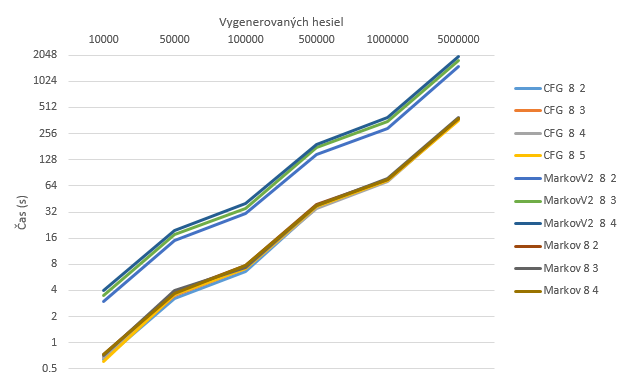
\includegraphics[width=1\textwidth]{generateTime}
    \caption{Čas generovania hesiel}
    \label{fig:generateTime}
\end{figure}

\section{Pamäťové nároky}
Popri meraní času, ktorý algoritmy strávia generovaním pevne daného počtu hesiel sme sledovali maximálnu potrebnú pamäť pri tomto procese.

\paragraph{}
Ďalej sme taktiež porovnali množstvo pamäte, ktorú potrebuje Markovovský zdroj ak si pamätá kompletnú maticu prefixov a znakov abecedy s optimalizáciou, ktorú sme popísali v sekcii \ref{sec:Markov}. Na výslednom grafe \ref{fig:memOptimization} môžme vidieť, že pre slovník \emph{rockyou-withcount} potrebuje Markovovský zdroj s touto optimalizáciou o \(TODO\).

\section{Výstupné heslá}
\label{sec:pass}
Po overení časovej zložitosti generovania hesiel pomocou jednotlivých algoritmov sme skúmali rôzne vlastnosti vygenerovaných slovníkov s heslami. Cieľom týchto testov bolo ukázať výhody a slabiny jednotlivých algoritmov a spraviť ich vzájomne porovnanie v zmysle šancí na čo najrýchlejšie nájdenie hľadaného hesla.

\subsection{Heslá zo vstupného slovníka}
Ako prvé sme skúmali koľko hesiel zo slovníka gramatika vygenerovala po vygenerovaní určitého počtu hesiel. Na grafoch, ktoré boli výstupom tohto testu sme na vodorovnej osi znázornili počet hesiel vygenerovaných gramatikou v desiatkach tisícov hesiel zatiaľ čo na vertikálnej osi je percento hesiel slovníka, ktoré sa medzi nimi nachádzajú. Pri tomto teste sme nechali oba algoritmy generovať 100 miliónov hesiel k čomu bol použitý slovník \emph{rockyou-withcount} obsahujúci 13 331 008 rôznych hesiel dĺžky 12 a menej znakov.

\paragraph{}
Nižšie vidíme grafy znázorňujúce vývoj počtu vygenerovaných hesiel, ktoré sa nachádzajú v slovníku. Zatiaľ čo na obrázku \ref{fig:uniqMarkov} vidíme koľko unikátnych hesiel bolo vygenerovaných pomocou algoritmu využívajúceho Markovovské zdroje, tie následne ukazujú vyššie popísanú vlastnosť zaoberajúcu sa počtom vygenerovaných hesiel patriacich do vstupného slovníka.

\begin{figure}[ht]
    \centering
    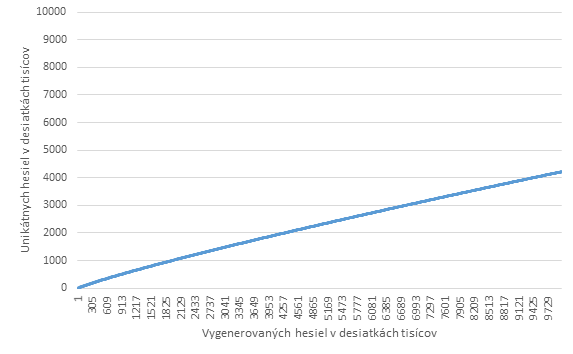
\includegraphics[width=1\textwidth]{uniqMarkov}
    \caption{Počet unikátnych hesiel}
    \label{fig:uniqMarkov}
\end{figure}
\paragraph{Heslá zo vstupného slovníka}
Na obrázku \ref{fig:sameDictAcc} vidíme priebeh hodnôt, kde heslá boli porovnávané so vstupným slonvíkom. Vidíme, že nami definované a implementované riešenie pomocou bezkontextových gramatík má na rozdiel od Markovovského zdroja omnoho pomalší rast počtu hesiel patriacich do slovníka. Pri 100 miliónoch generovaných hesiel to je niečo málo pod 700 tisíc.

\begin{figure}[ht]
    \centering
    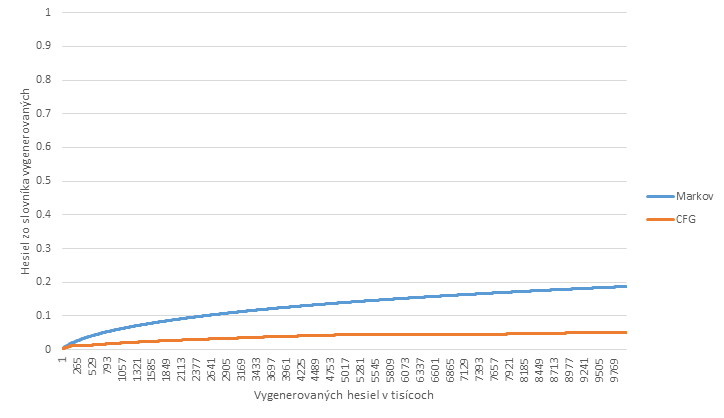
\includegraphics[width=1\textwidth]{sameDictAcc}
    \caption{Pomer vygenerovaných hesiel zo vstupného slovníka}
    \label{fig:sameDictAcc}
\end{figure}

\paragraph{Heslá z nezávislého slovníka}
Graf \ref{fig:otherDictAcc} znázorňuje hodnoty po porovnaní vygenerovaných hesiel s iným nezávislým slovníkom. Pri tomto teste sme zobrali heslá vygenerované našimi algoritmami, ktoré na vstupe dostali slovník \emph{rockyou-withcount}. Následne sme spravili testy počtu vygenerovaných hesiel, tentokrát avšak z iného ako vstupného slovníka. V tomto prípade sme použili slovník \emph{phpbb}. Týmto sme chceli ukázať schopnosť nášho algoritmu vygenerovať slovník veľmi podobný tým používaným v praxi.

\begin{figure}[ht]
    \centering
    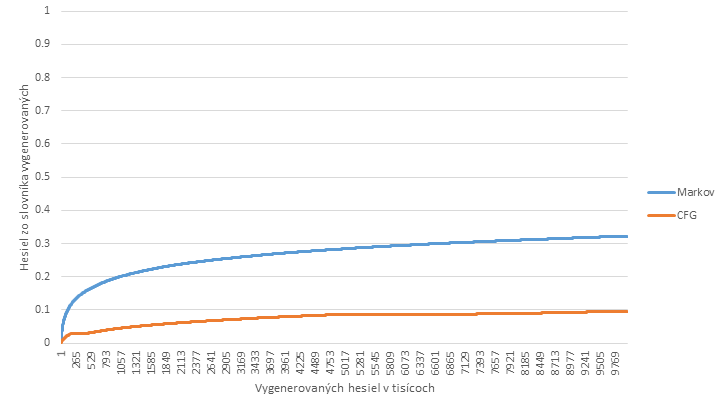
\includegraphics[width=1\textwidth]{otherDictAcc}
    \caption{Pomer vygenerovaných hesiel z nezávislého slovníka}
    \label{fig:otherDictAcc}
\end{figure}

\paragraph{}
Ďalej sme taktiež skúmali ako sa správajú nami implementované algoritmy ma menších dátach. Na obrázku \ref{fig:Acc6} je znázornený graf priebehu generovania hesiel, ktoré sa nachádzajú vo vstupnom slovníku. Na vodorovnej osi je ukázaný počet vygenerovaných hesiel, v tomto prípade to bolo 5 miliónov hesiel. Výška čiar určuje množstvo hesiel, ktoré boli nájdene vo vstupnom slovníku. Pre Markovovské zdroje sa toto číslo počíta z počtu unikátnych hesiel, ktoré boli vygenerované. Taktiež si môžme všimnúť, že algoritmus používajúci Markovovské zdroje je v tomto teste opäť lepší ako algoritmus používajúci pravdepodobnostné bezkontextové gramatiky. Opäť sme použili slovník \emph{rockyou-withcount} stiahnutý z nášho zdroja \cite{dictionaries}, ktorý sme upravili aby všetky heslá mali dĺžku najviac 6 znakov. Takto upravený slovník mal nakoniec 2 244 499 rôznych hesiel.

\begin{figure}[ht]
    \centering
    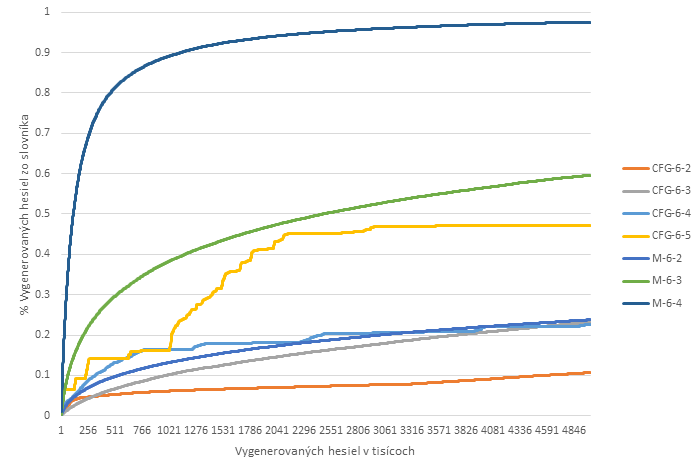
\includegraphics[width=1\textwidth]{sameDictAcc6}
    \caption{Počet vygenerovaných hesiel zo slovníka - dĺžka 6}
    \label{fig:Acc6}
\end{figure}

\pargraph{}
Graf \ref{fig:Acc7} zobrazuje namerané percentá pre nami implementované algoritmy spustené tak, aby generovali heslá s dĺžkou 7. Ako vstupný slovník bol použitý \emph{rockyou-withcount} upravený tak, aby obsahoval len heslá kratšie ako 8 znakov. Tento slovník obsahoval 4 752 979 unikátnych hesiel.

\begin{figure}[ht]
    \centering
    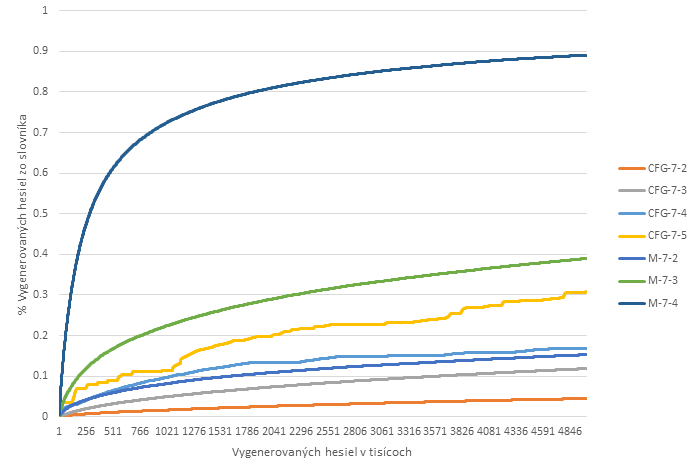
\includegraphics[width=1\textwidth]{sameDictAcc7}
    \caption{Počet vygenerovaných hesiel zo slovníka - dĺžka 7}
    \label{fig:Acc7}
\end{figure}

Nakoniec sme tento istý test opäť spustili na všetkých algoritmoch. Tentokrát vstupné parametre a slovník boli nastavené na generovanie hesiel maximálnej dĺžky 8. Takto upravený slonvík \emph{rockyou-withcount} obsahoval 7 717 387 hesiel z ktorých až 100 tisíc bolo vygenerovaných algoritmom používajúcim Markovovské zdroje s prefixom nastaveným na dĺžku 4. V grafe \ref{fig:Acc8} zobrazujúcom tieto dáta sme zobrazili výsledky tohto testu aj pre nami upravenú verziu Markovovských zdrojov, ktorá by mala byť schopná v konečnom čase vygenerovať heslá z celého priestoru možností. Označili sme ju ako \emph{M2-8-4} keďže sa jedná o druhú verziu Markovovských zdrojov použitých v tejto práci.

\begin{figure}[ht]
    \centering
    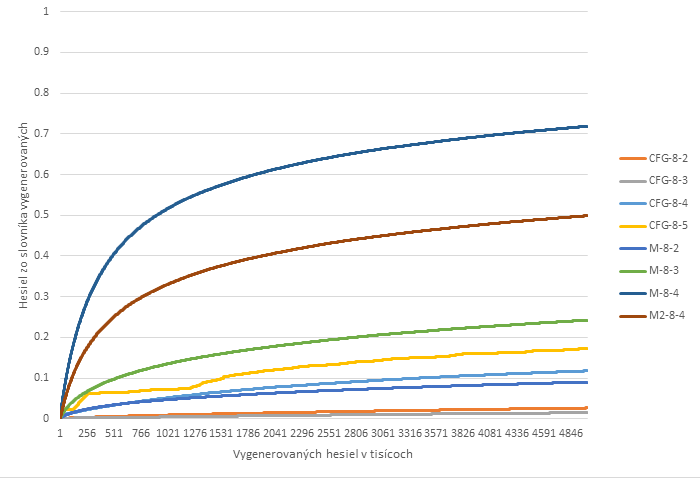
\includegraphics[width=1\textwidth]{sameDictAcc8}
    \caption{Počet vygenerovaných hesiel zo slovníka - dĺžka 8}
    \label{fig:Acc8}
\end{figure}

\paragraph{}
V prípade algoritmu, ktorý používa nami upravený Markovovský zdroj pri generovaní hesiel sme taktiež testovali vplyv nastavenia konštánt \(\delta\) a \(\varepsilon\). V nasledujúcom grafe \ref{fig:MarkovV2} zobrazujeme rozdiel v počte vygenerovaných hesiel zo vstupného slovníka pre jednotlivé parametre označené v legende grafu ako \(\delta-\varepsilon\). Vidíme, že tieto parametre nemajú žiaden vplyv na prvých 5 miliónov hesiel vygenerovaných týmto algoritmom.

\begin{figure}[ht]
    \centering
    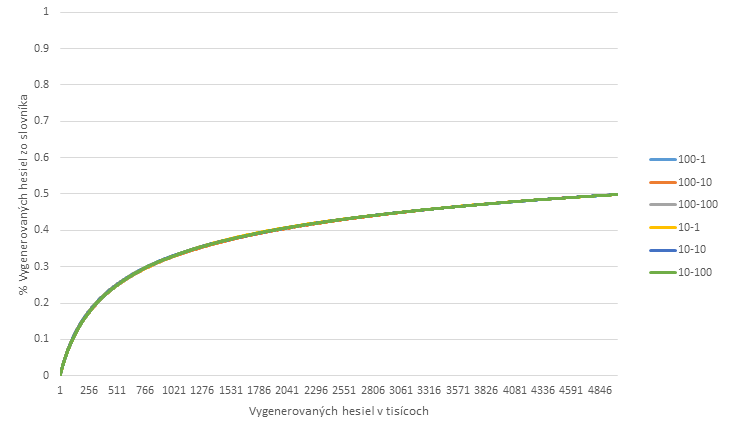
\includegraphics[width=1\textwidth]{sameDictAccMarkv2}
    \caption{Počet vygenerovaných hesiel zo slovníka pre rôzne hodnoty \(\delta\) a \(\varepsilon\) - dĺžka 8}
    \label{fig:MarkovV2}
\end{figure}

\paragraph{}
Na základe \ref{fig:sameDictAcc} a \ref{fig:otherDictAcc} vidíme, že nami navrhnutá metóda pomocou bezkontextových gramatík negeneruje veľa hesiel zo vstupného slovníka počas prvých miliónov vygenerovaných hesiel. Tento problém by sa dal vyriešiť tým, že by sme vždy ako prvé na výstup poslali všetky heslá zo slovníka, keďže ten býva zanedbateľne malý oproti veľkosti priestoru hesiel, ktorý musíme prehľadať aby sme definitívne našli hľadané heslo.

\subsection{Miery presnosti}
Pod týmto pojmom rozumieme metriky popisujúce nielen kvantitu nami generovaných hesiel patriacich do slovníka, ale snažia sa bližšie vyhodnotiť ako rýchlo sa gramatika dostane k heslám, ktoré boli podľa vstupného slovníka označené za najpravdepodobnejšie.

\paragraph{}
Stĺpce tabuľky \ref{mieryPresnosti} vyjadrujú hodnoty jednotlivých metrík pre daný algoritmus.
\begin{itemize}
	\item \emph{PPS} - Priemerná Pozícia v Slovníku - Vyjadruje priemernú pozíciu vo vstupnom slovníku pre heslá, ktoré boli vygenerované algoritmom na výstupe
	\item \emph{PPS \%} - Priemerná Pozícia v Slovníku - Vyjadruje percentuálnu pozíciu vrámci slovníku pre heslá, ktoré boli vygenerované algoritmom na výstupe
	\item \emph{RPSV} - Rozdiel Pozície v Slovníku a na Výstupe - Rozdiel v pozícii na vstupe a na výstupe algoritmu prenásobený percentuálnym počtom výskytov vo vstupnom slovníku
    \item \emph{OPSV} - Odchýlka Pozície v Slovníku a na Výstupe - Absolútna hodnota rozdielu v pozícii na vstupe a na výstupe algoritmu prenásobená percentuálnym počtom výskytov vo vstupnom slovníku
\end{itemize}

\[ \frac{\displaystyle\sum_{i=1}^{k}((indG_i - indS_x) * \frac{v_{ind_x}}{\sum_{j=1}^{n}v_j})}{k} \]

Vzorec vyjadrujúci mieru RPSV, kde \emph{n} vyjadruje počet hesiel vo vstupnom slovníku a \emph{k} je počet výskytov hesiel zo vstupného slovníka medzi generovanými. Hodnota \emph{\(indG_i\)} určuje poradie i-tého hesla vrámci generovaného slovníka. Hodnota \emph{\(indS_i\)} vyjadruje tú istú hodnotu pre vstupný slovník. Hodnoty \emph{\(v_i\)} sú počty výskytov hesiel zadefinované vo vstupnom slovníku.

\paragraph{}
Vzorec pre mieru OPSV je takmer identický s vyššie uvedeným vzorcom, jediný rozdiel je v absolútnej hodnote rozdielu medzi pozíciami na vstupe a na výstupe.

\[ \frac{\displaystyle\sum_{i=1}^{k}(|indG_i - indS_x| * \frac{v_{ind_x}}{\sum_{j=1}^{n}v_j})}{k} \]

\paragraph{}
Priemerná pozícia v slovníku ukazuje priemernú pozíciu vygenerovaných hesiel vo vstupnom slovníku. Keďže toto číslo je závislé od veľkosti vstupného slovníka, prikladáme k nemu v druhom stĺpci jeho percentuálnu hodnotu. Hodnoty d a p vyjadrujú maximálnu dĺžku hesiel v slovníku a dĺžku použitých prefixov v Markovovskom zdroji. Pre hodnoty 6, 7, 8 parametru \emph{d} sme použili slovník \emph{phppbb} upravený na heslá relevantnej dĺžky. Pre hodnoty \emph{d} rovné 12 sme použili omnoho robustnejší slovník \emph{rockyou}, skladajúci sa z takmer 14 miliónov unikátnych hesiel.

\begin{table}[]
\centering
\caption{Miery presnosti}
\label{mieryPresnosti}
\begin{tabular}{lll|llll}
       & d  & p & PPS & PPS \% & RPSV  & OPSV\\ \hline
CFG    & 6  & 2 & 31328    & 56,1       & 36,567 & 36,671    \\
CFG    & 6  & 3 & 26358    & 47,2       & 37,749 & 37,762    \\
CFG    & 6  & 4 & 31033    & 55,6       & 19,673 & 19,725    \\
CFG    & 6  & 5 & 28554    & 51,2       & 21,397 & 21,484    \\
CFG    & 7  & 2 & 47454    & 53,6       & 26,489 & 26,531    \\
CFG    & 7  & 3 & 40343    & 45,6       & 25,831 & 25,848    \\
CFG    & 7  & 4 & 46739    & 52,8       & 16,648 & 16,700    \\
CFG    & 7  & 5 & 46718    & 52,8       & 21,715 & 21,804    \\
CFG    & 8  & 2 & 88521    & 61,6       & 16,139 & 16,199    \\
CFG    & 8  & 3 & 61113    & 42,5       & 22,384 & 22,436    \\
CFG    & 8  & 4 & 70500    & 49,0       & 15,028 & 15,071    \\
CFG    & 8  & 5 & 75570    & 52,5       & 14,749 & 14,865    \\
Markov & 6  & 2 & 25219    & 45,2       & 28,307 & 28,332    \\
Markov & 6  & 3 & 25959    & 46,5       & 14,815 & 14,840    \\
Markov & 6  & 4 & 27705    & 49,7       & 3,649 & 3,706    \\
Markov & 7  & 2 & 39090    & 44,2       & 21,289 & 21,323    \\
Markov & 7  & 3 & 40283    & 45,5       & 13,321 & 13,353    \\
Markov & 7  & 4 & 43232    & 48,8       & 4,700 & 4,757    \\
Markov & 8  & 2 & 61688    & 42,9       & 15,745 & 15,792    \\
Markov & 8  & 3 & 66401    & 46,2       & 9,701 & 9,748    \\
Markov & 8  & 4 & 68291    & 47,5       & 4,596 & 4,658    \\ \hline \hline
CFG    & 12 & 4 & 3781788    & 28,3       & 5,879 & 5,925    \\
Markov & 12 & 4 & 4609712    & 34,5       & 2,191 & 2,224   
\end{tabular}
\end{table}

\paragraph{}
Z tabuľky \ref{mieryPresnosti} môžme vidieť, že obom našim algoritmom prospieva navýšenie vstupnej informácie o heslách. Toto je vidieť ako na percentuálnych hodnotách priemernej pozície v slovníku, tak aj na rozdieloch pozícií medzi vstupným a vygenerovaným slovníkom. Hodnota rozdielov pozícií má vyjadrovať presnosť generovania hesiel v správnom poradí kedy algoritmus je odmenený znížením skóre ak sa mu podarí vygenerovať niektoré heslo skôr, než sa nachádza vo vstupnom slovníku. Posledná miera \emph{odchýlka pozície v slovníku} má vyjadrovať absolútny rozdiel pozícií oproti vstupnému slovníku bez ohľadu na to, či heslo bolo vygenerované skôr alebo neskôr ako vo vstupnom slovníku. Malý rozdiel týchto hodnôt naznačuje, že väčšina hesiel, ktoré boli generované našimi algoritmami bola vygenerovaná neskôr ako bol ich výskyt vo vstupnom slovníku.